Im Kapietel "`Installation"' sind sie schon mit dem PPLT Center in ber�hrung gekommen. In diesem Kapitel
werde ich ihnen einen tieferen Einbick in die Funktionsweise und die Bedienung des PPLT Centers
geben. 

Doch zun�chst starten sie bitte die PPLT Center Applikation. Klicken sie auf den Reiter
"`Benutzer Datenbank"'. Die sehen dort das Symbol einer Gruppe diese hei�t \texttt{Admin}.
Mit einem Doppelklick auf dieses Symbol �ffnen sie diese Gruppe. In dieser Gruppe befindet 
sich lediglich ein Benutzer mit dem Namen \texttt{admin}. Das Symbol des Benutzers ist rot 
hinterlegt. Das bedeutet, dass dieser Benutzer der Superuser oder Administrator ist.
Sie sollten jetzt das Passwort des Administrators �ndern. Dazu �ffnen sie mit der
rechten Maustaste ein Kontextmenu und klicken auf "`Passwort �ndern"'\footnote{Siehe 
Abbildung \ref{fig:chadminpass}}. Es �ffnet sich ein Dialog, mit dem sie das Passwort 
�ndern k�nnen. 
\begin{figure}[ht]
	\centering
	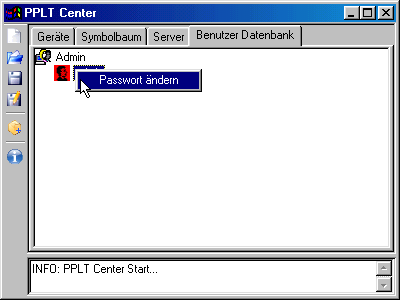
\includegraphics[scale=0.5]{chadminpass.png}
	\caption{Passwort des Administrators �ndern.}
	\label{fig:chadminpass}
\end{figure}

An dieser Stelle m�chte ich sie auf das eher eigenwillige Bedienkonzept des PPLT Centers
hinweisen. Wie sie sicher schon bemerkt haben, besitzt dieses Program kein Men�. Alle
aktionen werden mittels Kontextmen� initiert. Dieses �ffnen sie mit der rechten Maustaste.

\section{Allgemenies zur Oberfl�che}
Die Bedienoberfl�che des PPLT Centers besteht aus 3 Teilen. Dem ToolBar auf der 
linken Seite, mit dem sie eine Sitzung laden oder speichern k�nnen oder Module
installieren k�nnen. Der Zweite Teil ist das Log-Fenter,im unteren Teil des Programmes,
welches die (Fehler-)Meldungen der Bibliotek zeigt. Der Letzte und wichtigste Teil sind
die Reiter. Sie stellen die 4 Bereiche der PPLT dar. Zum einen die Ger�te und Server,
die sie laden und entladen k�nnen. Zum anderen der Symbol-Baum, in dem die Symbole 
verwaltet werden. Und zu letzt die Benutzerdatenbank mit der sie Benutzter und Gruppen
verwalten k�nnen. 

Im folgenden will ich mich auf die Bedienung und Funktion dieser Reiter beschr�nken. 
Dabei werde ich versuchen die Funktionsweise der PPLT anhand einiger Beispiele zu erkl�ren. 




